%TODO quitar schema por esquema

\chapter{Introducción}
\section{Objetivos}

Las facilidades que ofrece la federación de identidad son más que
evidentes, y podría ser interesante en muchos casos, tener estas
facilidades para otros servicios que requieran autenticación.

El principal objetivo de este proyecto es llevar las facilidades de la
gestión de identidad del ámbito de la web a otros servicios, como por
ejemplo el SSH. En este proyecto nos hemos centrado en integrar la
federación de identidad con el acceso por SSH, y puede servir como
prueba de concepto a la hora de llevar la autenticación por federación
de identidad a servicios diferentes de la web.

Las características más importantes de la federación de identidad, que
nos serán útiles en el SSH son:
\begin{enumerate}

    \item \textbf{Acceso a recursos de otras entidades}: La base de la
    federación de identidad es poder acceder a recursos de otra
    entidad con la misma cuenta con la que accedes a los recursos o
    servicios de tu propia entidad.

    \item \textbf{Gestión de identidad distribuida}: Al encargarse
    cada entidad de la federación de sus propios usuarios, y
    basándonos en las relaciones de confianza de la federación, se
    puede dar servicio a un mayor número de usuarios gestionando tan
    solo una pequeña cantidad de ellos. Esto puede crear algún tipo de
    duda, puesto que se pierde el control sobre los usuarios, pero no
    hay que olvidar que la federación es una red de confianza, donde
    cada entidad debe confiar en las demás, y para ello hay mecanismos
    seguros, como por ejemplo los certificados.

    \item \textbf{Unicidad de contraseña}: La federación de identidad
    nos brinda la posibilidad de acceder a diferentes servicios, que
    requieren autenticación, con la misma cuenta y la misma
    contraseña, y sin necesidad de replicar esta en los diferentes
    servicios, sino estando en tu propia entidad, incrementando así la
    seguridad de la misma, y la comodidad a la hora de cambiar de
    contraseña, o de nombre de usuario.
    %TODO problemas de las contraseñas únicas

    \item \textbf{Login único}: También se busca implementar el Single
    Sing On(SSO) para el SSH sobre federación, de tal forma que un
    usuario sólo tenga que autenticarse una vez, y a partir de ahí,
    tener acceso, sin necesidad de introducir ningún tipo de
    contraseña, a todos los servidores SSH disponibles.

\end{enumerate}

Por otra parte, hemos elegido llevar la federación al servicio SSH
porque es ampliamente utilizado, además de que ofrece una gran
potencia y versatilidad, abriendo así la puerta a la utilización de
otros servicios de forma fácil.

Por ejemplo, en el ambiente académico, puede ser interesante dar
acceso a un servidor SSH a todos los alumnos de Informática, bien sea
para que utilicen un supercomputador, o para que tengan una cuenta
dónde hacer las practicas. Dentro del objetivo de este proyecto
entraría delegar la gestión de estos usuarios a la federación,
facilitar así el proceso, 

% TODO revisar esto
así como por parte del alumno, como por
parte del administrador de las máquinas.

\newpage
\section{Caso de uso}

    En el siguiente caso de uso se muestra el funcionamiento básico del
    sistema, así como una serie de detalles que serán explicados
    detalladamente en la sección ``Implementación y despliegue''
    [\ref{implementacion}].

    %\textbf{Caso de uso del proyecto SSH sobre federación de identidad}:

    \begin{itemize}

    \item \textbf{Descripción}:
    
    La federación está pensada para aplicaciones web, pero sería
    interesante poder utilizar estos mecanismos para aplicaciones que
    autentican de otra manera diferente.

    %TODO revisar los tu
    En el caso del ssh federado intentamos llevar el concepto de hacer
    login una sola vez, y en tu entidad, al acceso por ssh. Buscando poder
    acceder por ssh a diferentes máquinas sin tener que escribir usuario y
    contraseña, una vez nos hayamos autenticado.  A través de ssh se pueden
    hacer muchas más cosas, como por ejemplo túneles ssh, port-forwarding,
    etc.

    \item \textbf{Proceso de Autenticación}:
    \label{casouso}

    \begin{enumerate}

        \item Se accede a una página especifica, protegida tras un SP.

        \item El usuario se autentica en la federación, y puede ver la
        página.

        \item Esta aplicación web intentará conseguir la clave RSA publica
        del usuario a través de los datos que manda la federación.

        \item Una vez autenticado en esa aplicación web, el usuario puede
        acceder a las cuentas ssh federadas de las que disponga sin tener
        que introducir password.

    \end{enumerate}

    Se puede ver un esquema del funcionamiento de este proceso en la figura
    \ref{fig:casodeuso}

    \item \textbf{Proceso de Autenticación alternativo}:
    La clave publica que recibe la aplicación a través de la federación
    será la de la máquina habitual del usuario. En caso de estar utilizando
    otra máquina es posible utilizar otra clave temporalmente.

    \begin{enumerate}

        \item Se accede a una página especifica, protegida tras un SP.

        \item El usuario se autentica en la federación, y puede ver la página.

        \item En la aplicación web se introduce la clave publica RSA temporal,
        para esta sesión.

        \item Una vez autenticado en esa aplicación web, el usuario puede
        acceder a las cuentas ssh federadas de las que disponga sin tener que
        introducir password.

    \end{enumerate}

    %TODO quitar del caso de uso
    \item \textbf{Implementación}:
    Para la implementación se ha optado por utilizar el mecanismo de acceso
    por clave publica-privada que nos ofrece el mismo protocolo ssh.
    Este mecanismo es el siguiente:
    El usuario crea un par de claves, para la máquina en la que se
    encuentra (ssh-keygen).

    Para dar acceso remoto sólo necesitamos conocer la clave publica
    (\$HOME/.ssh/id\_rsa.pub).
    
    Para poder acceder es necesario que el usuario disponga de su par
    privado.
    
    El servidor openssh, mira en el directorio personal del usuario, y
    busca en el archivo authorized\_keys (\$HOME/.ssh/authorized\_keys), antes
    de pedir password. Si encuentra alguna clave, intenta la autenticación
    por RSA, que es automática, sin petición de password. Por lo tanto
    nuestro objetivo es utilizar este servicio, pero en lugar de mirar en
    un archivo local, preguntaremos a un servidor remoto.
    
    \item \textbf{Requisitos}:

    Para poder acceder a cualquier máquina remota por ssh, en el servidor
    se debe poner el sshd parcheado. Además se debe crear una cuenta de
    usuario. Es recomendable el deshabilitar la posibilidad de cambiar el
    password, puesto que si se puede cambiar el password de la cuenta, es
    posible acceder a esta sin pasar por la federación. También es
    conveniente no permitir la creación, o borrar, los ficheros dentro de
    .ssh del home del usuario, por la misma razón que lo anterior.

    También será necesario definir un esquema para la federación, que añada
    el campo ssh\_rsa\_public\_key, si queremos que el acceso sea lo más
    automatizado posible.

    %TODO quitar del caso de uso
    \item \textbf{Temas a discutir}:

    \begin{enumerate}
        \item Tipo del servidor de claves, LDAP, base de datos, etc

        \item Posibilidad de cambiar password, y permisos en la cuenta previamente creada.
    \end{enumerate}

    \end{itemize}

    \begin{figure}[htp!]
        \centering
            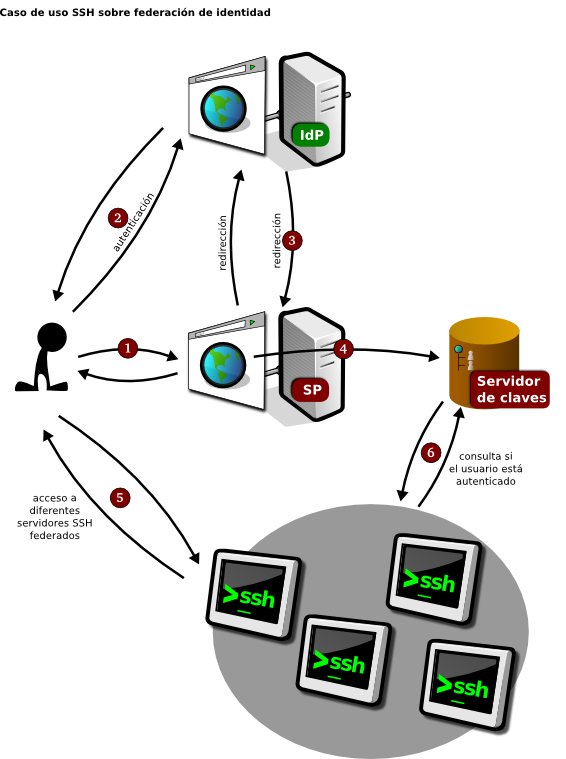
\includegraphics[width=\textwidth]{img/casodeuso1.png}
            \caption{Caso de Uso}
        \label{fig:casodeuso}
    \end{figure}

    Para una mayor compresión de la figura \ref{fig:casodeuso} vamos a
    explicar cada paso de manera un poco más exaustiva:

    \begin{itemize}
        
        \item{Paso 1:} Antes de poder acceder a cualquier servicio de
        ssh federado, el usuario tendrá que autenticarse. Para ello se
        utilizan los mecanismos que ofrece la federación de identidad.
        Por tanto el usuario intentará acceder a una aplicación web,
        protegida tras un Service Provider (SP) de la federación de
        identidad.

        %TODO quitar esto, puede haber tantos SP como se quiera
        Este SP no tiene por qué pertenecer a ninguna de las entidades
        que forman la federación, sino que será un único servidor
        central.

        \item{Paso 2:} Según el funcionamiento de la federación, si el
        usuario no está aún autenticado en la federación de identidad,
        el SP, redireccionará al usuario hacia una aplicación WAYF
        (where are you from), dónde seleccionará su entidad de origen,
        y tras esto será redirigido al Proveedor de Identidad (IdP) de
        su entidad. En esta aplicación web será donde el usuario
        proporciona sus credenciales, siendo esta una operación
        segura, puesto que el IdP está gestionado por nuestra propia
        entidad, y por lo tanto, no estamos proporcionando nuestra
        contraseña a ninguna otra entidad.

        \item{Paso 3:} Una vez autenticado en la federación de
        identidad, el sistema redirigirá al usuario al SP al cuál
        quería entrar en un principio, pasándole a este los datos
        necesarios para asegurar la identidad del usuario.
        Aunque este proceso pueda parecer largo, para el usuario son
        un simple par de clicks, puesto que todo el trabajo se realiza
        automáticamente por la federación.

        \item{Paso 4:} La aplicación principal, tras el SP, recibirá
        entonces los datos necesarios del usuario, que le serán
        proporcionados por el IdP de la entidad de este. Y con estos
        datos creará una entrada en el servidor de claves, el cuál
        será consultado por los servidores ssh para verificar que el
        usuario esté autenticado en la federación.
        En este paso es donde se comienza a sacar la federación de
        identidad del ámbito web, teniendo un lugar dónde se
        almacenarían los usuario autenticados, con un sistema
        diferente al de cookies.

        \item{Paso 5:} El usuario ya está autenticado, y ahora puede
        entrar en uno o varios servidores ssh federados sin necesidad de
        escribir su contraseña. Por supuesto tendrá un tiempo límite,
        la sesión expirará dado un cierto tiempo.

        \item{Paso 6:} El servidor ssh tiene que saber si el usuario
        que intenta acceder está autenticado en la federación, por lo
        que consultará el servidor de claves, para confirmar que dicho
        usuario está autenticado, y además es quien dice ser.

    \end{itemize}

%TODO importancia del SSH, túneles, importación X

\newpage
\section{Antecedentes}

    La federación de identidad es un concepto relativamente nuevo, y
    por tanto hoy en día hay pocas federaciones funcionando.

    La federación de identidad de universidades andaluzas está
    naciendo ahora mismo, por lo tanto se está nutriendo de la
    experiencia de otras federaciones con algo más de tiempo.

    Una de las federaciones más activas en lo que se refiere a
    investigación y desarrollo de aplicaciones para la federación de
    identidad es la federación noruega, \textbf{feide}.

    El proyecto de SSH sobre federación de identidad nace a partir de
    un documento publicado el 20 de agosto de 2007 por la federación
    noruega.

    \href{http://rnd.feide.no/content/feide-and-ssh-secure-shell}{http://rnd.feide.no/content/feide-and-ssh-secure-shell}
    %\textbf{http://rnd.feide.no/content/feide-and-ssh-secure-shell}

    Este documento investiga como las credenciales de la federación
    de identidad pueden ser usadas para autenticar a diferentes
    servicios, como el SSH.

    A partir de esta idea se proponen diferentes formas de conseguir
    la autenticación de SSH sobre la federación de identidad.
    Este proyecto se basa en las ideas propuestas por la federación
    noruega, dando un paso más, e intentando automatizar al máximo el
    proceso, para dar una mayor comodidad al usuario, y también al
    administrador.

    Todos los métodos propuestos en este documento se basan en la
    utilización de un navegador web para obtener las credenciales
    de autenticación del servicio SSH. Primero el usuario entra en
    una página web del proveedor de servicio SSH (SP). Como no está
    autenticado aún, se le muestra una página por defecto de
    bienvenida. Luego el usuario se autentica a través del
    proveedor de identidad (IdP).

    Como se puede observar en el caso de uso \ref{casouso}, este es el
    método que hemos utilizado en el proyecto de SSH sobre federación
    de identidad. Hemos mantenido la misma idea de autenticación
    propuesta por la federación noruega.

    En este documento se propone colocar una página web, tras un SP,
    por cada servidor SSH federado que se ofrezca. En nuestro caso no
    hemos mantenido esta idea, puesto que complicaría el
    despliegue del servicio.

    A continuación vamos a detallar las diferentes propuestas que se
    pueden encontrar en este documento, además comentaremos los pros y
    los contras de estas ideas.

    \begin{itemize}
        
        \item{One-time passwords. Contraseñas de un solo uso:}
        Este método consiste en generar una contraseña de un solo uso
        para el usuario. Este es un método sencillo en el cual cada
        vez que un usuario se autentica, se generaría una cuenta con
        una contraseña aleatoria, valida solo una vez.

        Para este caso se puede utilizar OPIE (one-time password in
        everything), que es una aplicación desarrollada por el
        laboratorio de investigación naval de los Estados Unidos de
        América. Se puede utilizar en el servidor web el ejecutable
        ``opie-client'' para generar las contraseñas para los
        usuarios.

        Con este sistema, la contraseña generada sólo será valida una
        vez. Después de esto no podrá ser usada otra vez para
        autenticarse en este servidor.

        Este método es de fácil implementación, pero tiene grandes
        inconvenientes. El principal inconveniente es que es muy
        incomodo para el usuario, ya que tiene que ir copiando y
        pegando la contraseña para poder acceder.

        Otro gran inconveniente es que se pierde la posibilidad de
        Single Sign On (SSO), puesto que por cada servidor SSH tendrás
        una contraseña diferente.

        En cambio solventa el problema de tener que introducir tu
        contraseña en un servidor extraño, puesto que la contraseña
        que se introduce es de un solo uso.

        \item{Credenciales de la federación:} 
        Otra posibilidad es proporcionar nuestras credenciales de la
        federación de identidad directamente sobre el servidor SSH,
        sin pasar a través del la autenticación web. Esta solución
        puede ser implementada usando un pequeño módulo PAM, que se
        conecta a la federación y autentica al usuario directamente
        con las credenciales que este ha proporcionado.

        Pero este método no es una solución viable, puesto que el
        nombre de usuario y la contraseña nunca debería pasar a través
        de un proveedor de servicio.

        \item{Clave pública:}
        Una mejor opción es autenticar al usuario usando criptografía
        de clave pública. Primero el SP puede intentar obtener la
        clave pública del usuario a través de los atributos recibidos
        del IdP.
        
        Si la clave pública no se proporciona por parte del IdP, se
        puede ofrecer al usuario la posibilidad de subir la suya a
        través de una interfaz web. La clave se almacenará en el
        fichero authorized\_keys, permitiendo al usuario autenticarse
        usando su clave privada.

        Hay que tener en cuenta que si no se borra la clave del
        fichero authorized\_keys, el usuario podrá entrar directamente
        sin tener que autenticarse en la federación de identidad. Esto
        se podría solventar con un proceso cron que limpiara los
        fichero cada cierto tiempo.

        Este método es en el cuál nos hemos basado de una manera más
        directa, puesto que ofrece al usuario una autenticación mucho
        más simple, y solventa la mayoría de los problemas.

        La aplicación web tras el SP que hemos desarrollado es igual a
        la descrita en el documento. En un principio intenta conseguir
        la clave pública a través de los atributos que proporciona el
        IdP, pero también ofrece la posibilidad de introducir una
        manualmente.

        Sin embargo, aunque solventa el problema de tener que recordar
        una clave, y otros problemas relacionados con el uso de
        contraseñas, no es una solución completa. Al estar ligada a un
        solo servidor SSH no es posible entrar en diferentes
        servidores con una sola autenticación, sino que habría que
        autenticarse en cada uno de ellos. Esa parte es la que aporta
        nuestro proyecto.

        \item{Java SSH aplet:}
        Otra opción propuesta en el documento de la federación noruega
        es el uso de un servicio web, tras un SP, que lanza un applet
        SSH en Java. Se puede ofrecer un login automático.

        En este caso se realiza la operación inversa a lo que se busca
        en el proyecto, pero con similar resultado. En un principio
        queremos llevar los beneficios de la federación de identidad
        fuera del ámbito web, pero buscando este objetivo hacemos lo
        opuesto, y es llevar otro ámbito, como es el del SSH a la Web,
        mediante el uso de un applet de Java.

        Lo bueno de este método es que tiene acceso a cuentas SSH de
        manera más simple aún, puesto que funcionaría de igual manera
        que cualquier página web federada. Además sigue estando la
        posibilidad de entrar en diferentes servicios SSH, habiendo
        realizado la autenticación una sola vez.


        %TODO segunda persona
        Lo malo es que no te da un acceso SSH completo, sino que te
        ofrece una shell, pero siempre a través del navegador, con las
        limitaciones que esto conlleva. Además de que no aporta nada a
        la idea de llevar la federación de identidad fuera de la web.

    \end{itemize}

    En conclusión podemos decir que hay algunas investigaciones
    previas sobre el concepto de SSH sobre federación de identidad, y
    que la idea de realizar este proyecto nace, en gran medida, a
    partir del documento publicado por la federación noruega.
    
    %TODO revisar esto
    Por supuesto nuestro proyecto no se queda en una prueba de
    concepto, como es el caso del documento comentado, sino que se a
    partir de estas pruebas de concepto se implementa un sistema
    más completo y funcional, el cuál utiliza y mejora las ideas
    propuestas, dando así un nuevo punto de vista a la idea principal.

    
    \subsection{Otros antecedentes a destacar}
    
        Como se verá en el capitulo \ref{openssh}, para la
        implementación hemos optado por crear un parche para el
        servidor SSH openssh, para realizar la autenticación por clave
        pública a través de un servidor externo, además de por los
        ficheros authorized\_keys.

        Por ello es interesante comentar en esta sección un proyecto
        que realiza algo similar a nuestra implementación.

        \href{http://dev.inversepath.com/trac/openssh-lpk}{http://dev.inversepath.com/trac/openssh-lpk}
        %\textbf{http://dev.inversepath.com/trac/openssh-lpk}

        Este proyecto consiste en un parche para el servidor SSH
        openssh, que nos da la posibilidad de autenticar a los
        usuarios a través del sistema de clave pública, almacenando
        las claves en un servidor LDAP.

        ``The lpk patch allows you to lookup ssh public keys over LDAP
        helping central authentication of multiple servers. This patch
        is an alternative to other authentication system working in a
        similar way (Kerberos, SecurID, etc...), except the fact that
        it's based on OpenSSH and its public key code.''
        
        Para este proyecto buscábamos algo parecido, pero en un
        principio no nos queríamos restringir al uso de un servido
        LDAP. Aunque posteriormente nos hemos basado en este protocolo
        para proporcionar el servidor de claves.

        Sin embargo no nos hemos decantado por usar este parche, por
        su complejidad, y hemos decidido implementar uno nuevo, con
        las mínimas variaciones posibles, y que cubriera nuestro caso
        específico.

        El parche implementado, es fácilmente modificable para que
        permita diferentes servidores de claves, no solo servidores
        LDAP.
